\section{Artificial Immune Systems (AIS)} \label{sec:bgais}

The primary goal of the Biological Immune System (BIS) is to protect the body from potentially harmful material \cite{AISSOA2015}. It is composed by a multilevel defense mechanism that is capable of distinguishing between molecules from the body itself and foreign ones, selecting a specific response to a threat, and enacting an inflammatory reaction in order to maintain the health and safety of the body. All of these activities are capable of evolving through time since they rely on aspects of learning and memory, which are present in the BIS.

In 1986, Farmer et al. \cite{ImmuneSysAdapML1986} sought inspiration in the properties and theories of this biological system to propose a computational model, named Artificial Immune System (AIS). It was built in such a way that the immunological concepts and processes are distilled into algorithms that can be simulated by a computer in order to solve all sorts of problems from the real world. The idea behind it is that, since this system is able to protect us, it might be computationally useful \cite{EvaluateAIS2005}. Nevertheless, by that time, the resources available were not powerful enough to allow its usage in real systems \cite{AdaptiveImmunitySAS2021}.

Recently, the advances in technology enabled complex tasks to be performed in a fast and efficient way. This provided the researchers the tools needed to implement and further improve the application of the immunological concepts into a wide range of problems. For example, AIS techniques have been used in problems like anomaly detection, optimization, classification and clustering \cite{AISSOA2015}. The Negative Selection, along with the Clonal Selection, Immune Network Theory and the Danger Theory are amongst the most researched approaches in the literature \cite{NSAResearch2021}.

This section is structured as follows: initially, the main concepts of the Biological Immune System will be laid out. Then, the Negative Selection algorithm will be explained in depth, for it will be exercised throughout this work.

\subsection{Overview of the Biological Immune System}

As mentioned previously, the Artificial Immune System is a model inspired by its biological counterpart in order to solve computational problems. Therefore, there is a need to introduce the main concepts and processes found in the Biological Immune System so that the analogies and metaphors implemented by the AIS might be better understood. This subsection focuses on providing the reader with the foundational knowledge on the BIS. 

\subsubsection{Main Concepts}

Immunity can be defined as the ability to respond to unknown substances \cite{ICBook2009}. In this sense, the Biological Immune System (BIS) comprises a set of structures and mechanisms which are capable of distinguishing the body's cells from foreign substances and responding adequately. It includes specific organs, cells and molecules. It is a complex, fault-tolerant and distributed multilevel defense mechanism composed of two main layers, namely the innate immunity and the adaptive immunity \cite{Kuby2019}. 

The innate immunity is the body's first line of defense. Inherited from the host's progenitors, it is responsible for a quick or immediate response against infections. It is achieved through physical and chemical barriers or through cellular responses. The barriers are considered nonspecific mechanisms that work as shields against pathogens by blocking them from entering the body. They comprise the skin, mucous membranes on the body's openings and the secretions of both. The low pH of the skin, for instance, inhibits the proliferation and growth of bacteria, while the antimicrobial substances present in saliva and tears keep the antigens from invading through the membranes \cite{ICBook2009}. The cellular response, on the other hand, focus on perceiving the pathogens that were able to surpass the barriers and activating a variety of cellular responses, which include: the ingestion of the substance (phagocytosis), the induction of an inflammatory response and the triggering of the adaptive immunity for a tailor made response. 

The adaptive immunity is an immunological mechanism that is capable of "specifically recognize and selectively eliminate foreign microorganisms and molecules" \cite{ICBook2009}. In contrast with the innate immunity, it has a high level of specificity when dealing with the antigens, meaning that the response is customized and based on the particularities of the foreign substance. The downside is that the response can take days to be performed. Nevertheless, the information from previous infections is persisted in order to achieve a faster response when a similar antigen is detected. In the literature, the adaptive immunity responses is divided into two distinct, but overlapping, categories: the humoral immunity and the cellular immunity.

The first kind of response, called humoral immunity, relies on the interaction between the antigen and B lymphocytes, a specific type of white blood cell also known as B Cell. These cells are created in the bone marrow and, when activated, are able to produce antibodies, which bind to the antigen during the immunological response as a means to destroy it. This can only happen if there is a match between the antibody and the surface of the foreign material. Humans are thought to have \(10^7\) to \(10^8\) different antibodies with distinct chemical compositions \cite{ImmuneSysAdapML1986} that account for the possible variations of antigens that one may find during the course of a lifetime.

The second kind of adaptive response is called cellular immunity and is mediated by lymphocytes called T cells. These cells are also produced in the bone marrow, but are matured in an organ named Thymus. They are responsible for killing tumor cells and cells from the body that were infected by the pathogen (altered self-cells).

\subsubsection{Overview of the Immune Response}

\begin{figure}[!h]
	\centering
	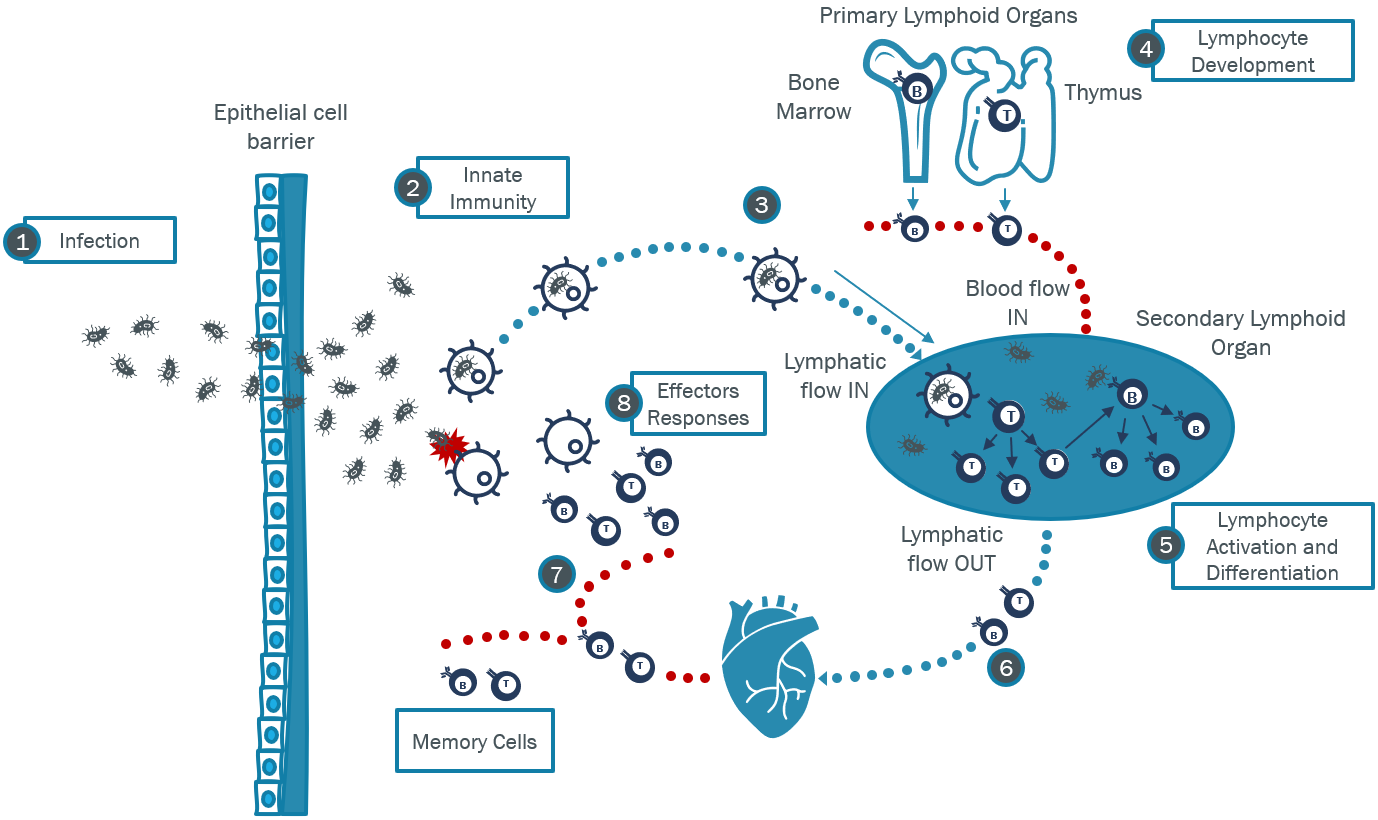
\includegraphics[width=0.9\textwidth, keepaspectratio]{img/overview_bis.png}
	\caption{Main Processes of an Immune Response~\cite{Kuby2019}}
	\label{fig:BISOverview}
\end{figure}

Figure \ref{fig:BISOverview} shows an overview of the main activities that may happen during an immune response. The whole process starts with an infection caused by an antigen that was capable of passing through the physical and chemical barriers of the body (1). After that, when the pathogen is detected by the front line phagocytic cells, a hormone-like protein called cytokine is released by them as to induce a local inflammatory response (2). Besides that, these cells are capable of engulfing the antigen and transporting it through the lymphatic vessels with the objective of enacting the adaptive immune response (3).

In the meanwhile, both B and T lymphocytes are derived in the Bone marrow via a process called hematopoiesis. The receptors of these cells undergo a pseudo-random genetic rearrangement process during their creation that account for the variety of cells, and thus the ability to bind with unseen substances \cite{AIS2014}. While the B cells flow directly through the blood flow into secondary lymphoid organs, the T cells stop at the Thymus to be matured, and then follow the same path as the B cells (4). The maturation of the T cells is a censoring process in which the lymphocytes are tested against proteins of the body. If a T-cell strongly binds to some self-protein, it is discarded. Hence, only the T-cells that did not have a strong bind are allowed to flow through the bloodstream and be used against the pathogen. This process is called Negative Selection and aims at avoiding autoimmune responses.

The adaptive immune response starts at a secondary lymphoid organ, with the arrival of the phagocytic cell carrying the antigen. In this step, a mechanism called Clonal Selection is performed (5). The B and T lymphocytes with a high level of engagement with the pathogen proliferate and mutate (somatic hypermutation) as a means to grow in number and to improve the affinity with the foreign substance. Afterwards, these differentiated cells leave the lymphoid organ and are pumped throughout the circulatory system by the heart (6) until reaching the local of the inflammatory response (7). Finally, the specialized lymphocytes act on the antigens in order to destroy the residual of the invasion (8). These cells are kept as memory cells so that, in the case of a future similar threat, allow for a faster response. 

\subsection{Negative Selection Algorithm} \label{sec:bgNS}

\subsubsection{Algorithm Overview} \label{sec:bgNSA}

\subsubsection{Detectors} \label{sec:bgNSADetectors}

\subsubsection{Matching Function} \label{sec:bgNSAMatching}
